\documentclass[12pt,a4paper]{scrartcl}
\usepackage{url, pdflscape}
\usepackage[final]{pdfpages}
\usepackage[colorlinks]{hyperref}
\usepackage{longtable}
\title{Student Robotics Risk Assessment Form}

\begin{document}
\maketitle

\begin{description}
\item[Activity being assessed:] Student Robotics Competition (25 - 26 April, 2015)
\item[Persons at risk:] Competitors, Team Leaders, Blueshirts, Newbury Racecourse Staff
\item[Location:] Newbury Racecourse Grandstand
\end{description}

\begin{description}
\item[Assessor's name:] Andrew Busse
\item[Responsible Persons:] Sam Phippen (SC - Events); Team Leaders
\item[Date of assessment:] \date{\today}
\end{description}
\clearpage

\newcommand{\risk}[4]{
 #1 & #2 & #3 & #4 \\
}

\begin{landscape}
\section{Risks}
The following risks have been considered for the Student Robotics Competition. 
Further description of the meaning of risk ratings (presented in this section as
$L \times S$) can be found in the next section.

This risk assessment is to be considered in addition to the Newbury Racecourse
Generic Risk Assessment (dated 23/03/2012)

\centering
\begin{longtable}{|p{17em}|p{8cm}|p{4cm}|p{4em}|}
\hline
\textbf{Hazard} & \textbf{Control Measures} & \textbf{Responsible Person} & \textbf{Risk Rating} \\
\hline
\endhead

\endfoot

\risk{Injury while using manual or power tools}
{Student Robotics will not provide any tools to competitors. All tools brought by Student Robotics will only
be used by SQEP Blueshirts, and will be safely stored when not in use.}
{SC - Events}
{4}

\risk{}
{Teams will bring their own tools - Team Leaders must ensure tools are fit for purpose, that students using the tools are competent, and are wholly responsible for their use.}
{Team Leaders}
{}
\hline

\risk{Interaction with robots: electric shock, minor injury}
{Team Leaders to supervise work on robots in team pits, Blueshirts will also intervene if work seems unsafe.
Food and Drink is not permitted in team pit areas.}
{SC - Events, Team Leaders}
{3}

\risk{}
{Robots subject to a safety inspection before entry into an arena. Arena access controlled by
Blueshirts - maximum of 4 teams at a time, and modification of robots inside the arena is banned.}
{SC - Events}
{}

\hline

\risk{Trip Hazard from trailing extension leads}
{Extension leads taped down and inspected regularly, kept away from walkways
where reasonably practicable. Blueshirts and Team Leaders to enforce teams
keeping within their areas and that areas are kept tidy}
{SC - Events, Team Leaders}
{1}
\hline

\risk{Battery failure - smoke, fire}
{Teams will hand over batteries and chargers on arrival, from this point
SQEP Blueshirts to handle battery charging in a designated area. Blueshirts
and Team Leaders to identify batteries showing signs of damage or swelling
and deliver to Helpdesk for safe disposal.}
{SC - Events, Team Leaders}
{4}
\hline

\risk{Injury due to objects falling from arena / arena components coming loose}
{Arena to be constructed and tested as per Method Statement, and will
be subject to inspection by Blueshirts throughout the event, with
interventions for repair if deemed necessary}
{SC - Events}
{3}
\hline

\end{longtable}
\end{landscape}

\begin{landscape}

\section{Assessment Guidance}

The risk ratings of the risks in the previous section are calculated by multiplying $L$, the likelihood rating, by $S$, the severity rating.

\bigskip
\begin{minipage}[b]{0.5\linewidth}
\begin{tabular}[c]{lc}
\hline
  \textbf{Likelihood} & \textbf{Likelihood rating} \\
\hline
  Very unlikely & 1 \\
  Unlikely & 2 \\
  Likely & 3 \\
  Fairly likely & 4 \\
  Very likely & 5 \\
\hline
\end{tabular}
\end{minipage}
\begin{minipage}[b]{0.5\linewidth}
\begin{tabular}[c]{lc}
\hline
  \textbf{Severity} & \textbf{Severity rating} \\
\hline
  First Aid injury/illness & 1 \\
  Minor injury/illness & 2 \\
  `3 day' injury/illness & 3 \\
  Major injury/illness & 4 \\
  Fatality/disabling injury & 5 \\
\hline
\end{tabular}
\end{minipage}
\bigskip

The following should be used to rate the risk and plan corrective action:
\bigskip
\newcommand{\riskinfo}[4]{
  #1 & #2 & #3 & #4 \\
}

\begin{tabular*}{\linewidth}[c]{cccp{33em}}
\hline
  \textbf{Risk Rating} & \textbf{Category} & \textbf{Tolerability} & \textbf{Comments} \\
\hline

  \riskinfo{1--2}{Very Low}{Acceptable}
  {No further action is necessary other than to ensure that the controls are maintained.}

  \riskinfo{3--4}{Low}{Acceptable}
  {No additional controls are required unless they can be implemented at very low cost (in terms of time, money and effort).}

  \riskinfo{5--7}{Medium}{Tolerable}
  {Consideration should be given as to whether the risks can be lowered, where applicable, to a tolerable level, and preferably acceptable level, but the costs of additional risk reduction measures should be taken into account.  The risk reduction measures should be implemented within a defined time period.}

  \riskinfo{8--14}{High}{Tolerable}
  {Substantial efforts should be made to reduce the risk.  Risk reduction measures should be implemented urgently within a defined time period and it might be necessary to consider suspending or restricting the activity, or to apply interim risk control measures, until this has been completed. Considerable resources might have to be allocated to additional control measures.}

  \riskinfo{15 and above}{Very High}{Unacceptable}
  {Substantial improvements in risk control are necessary, so that risk is reduced to a tolerable or acceptable level.}

\hline
\end{tabular*}

\end{landscape}


%\clearpage

%\newpage
%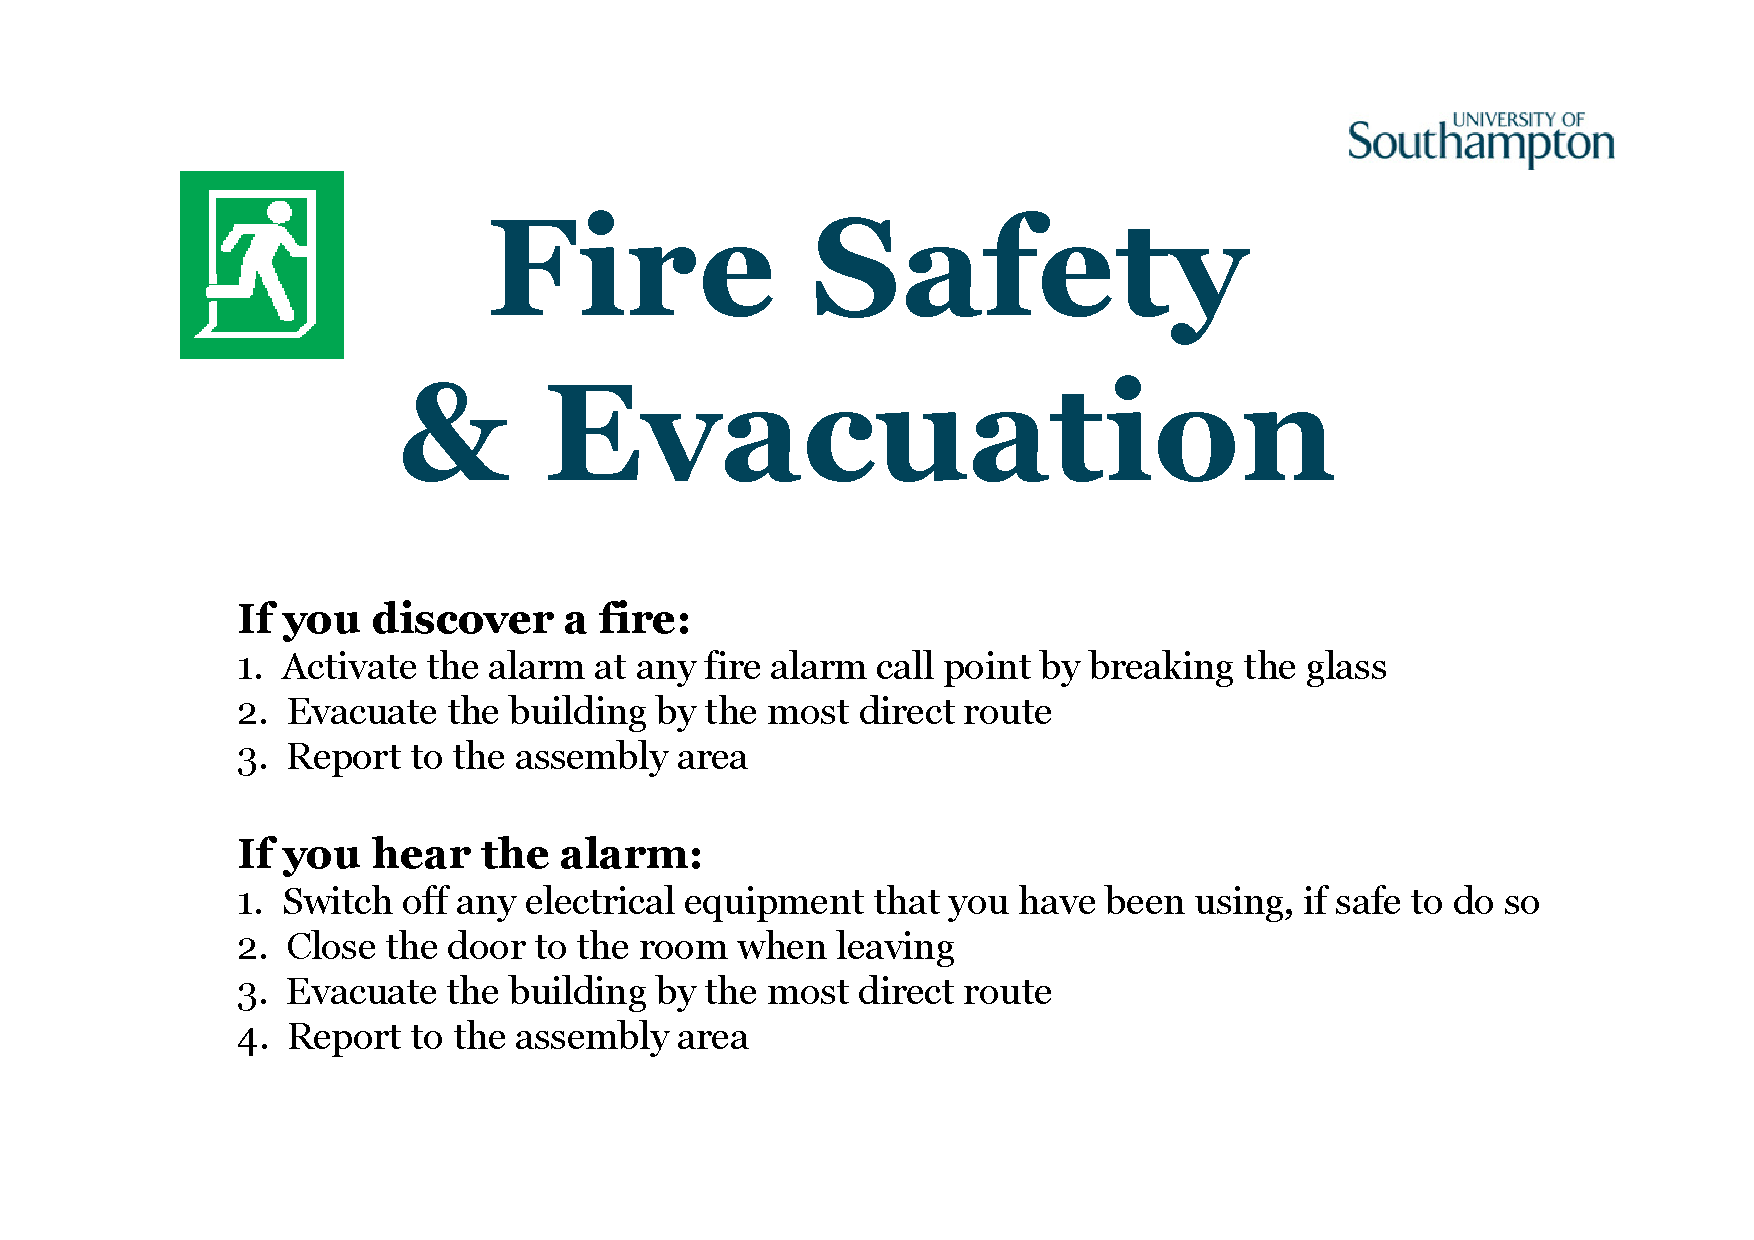
\includepdf[scale=1.0,landscape]{Fire1.pdf}

\end{document}

